\chapter{Testy środowiska symulacyjnego}
\label{sec:tests}
W tym rozdziale przedstawione są różne konfiguracje pakietów, wraz z wykresami ruchów platform, oraz wnioski płynące z tych zachowań.

Uruchomiono odpowiednią konfigurację pakietów i połączono je strumieniami konfiguracyjnymi.
Wiadomości przesyłane w odpowiednich strumieniach zostały zapisane do pliku za pomocą narzędzia
\texttt{rosbag}, dostępnego w środowisku ROS.
Za pomocą narzędzia \texttt{rostopic}, wyeksportowano dane z plików do pliku rekordów, gdzie każde pole oddzielone jest przecinkiem (\emph{Comma Separated Value}(CSV)).
Używając skryptu w programie Gnuplot, narysowano wykresy w formacie PDF, które następnie załączono poniżej.

\section{Weryfikacja działania modelu dynamiki}
	W tym teście porównano działanie modelu dynamiki oraz jej enkoderów w stosunku do zadanego sterowania.
	W tym celu uruchomiono scenę posiadającą dwa modele kinematyki i jeden dynamiki oraz obserwator symulacji, patrz rysunek \ref{uml:comparison}.
	Jeden model kinematyki użyto do przekształcania zadanych prędkości kół do prędkości liniowej i kątowej platformy, którą to za pomocą symulatora scałkowano w celu określenia zadanej trasy robota. Drugi model, korzystając z enkoderów, realizował mechanikę odometrii, wyznaczał trasę na podstawie danych o obrotach kół.
	Wiadomości, zawierające pozycje modeli w czasie, były zapisywane do pliku.
	Dodatkowo, wtyczka symulatora, obserwator symulacji, generowała dane porównujące odległość i kąt obrotu modeli od siebie.
	
	\begin{figure}[h]
		\centering
		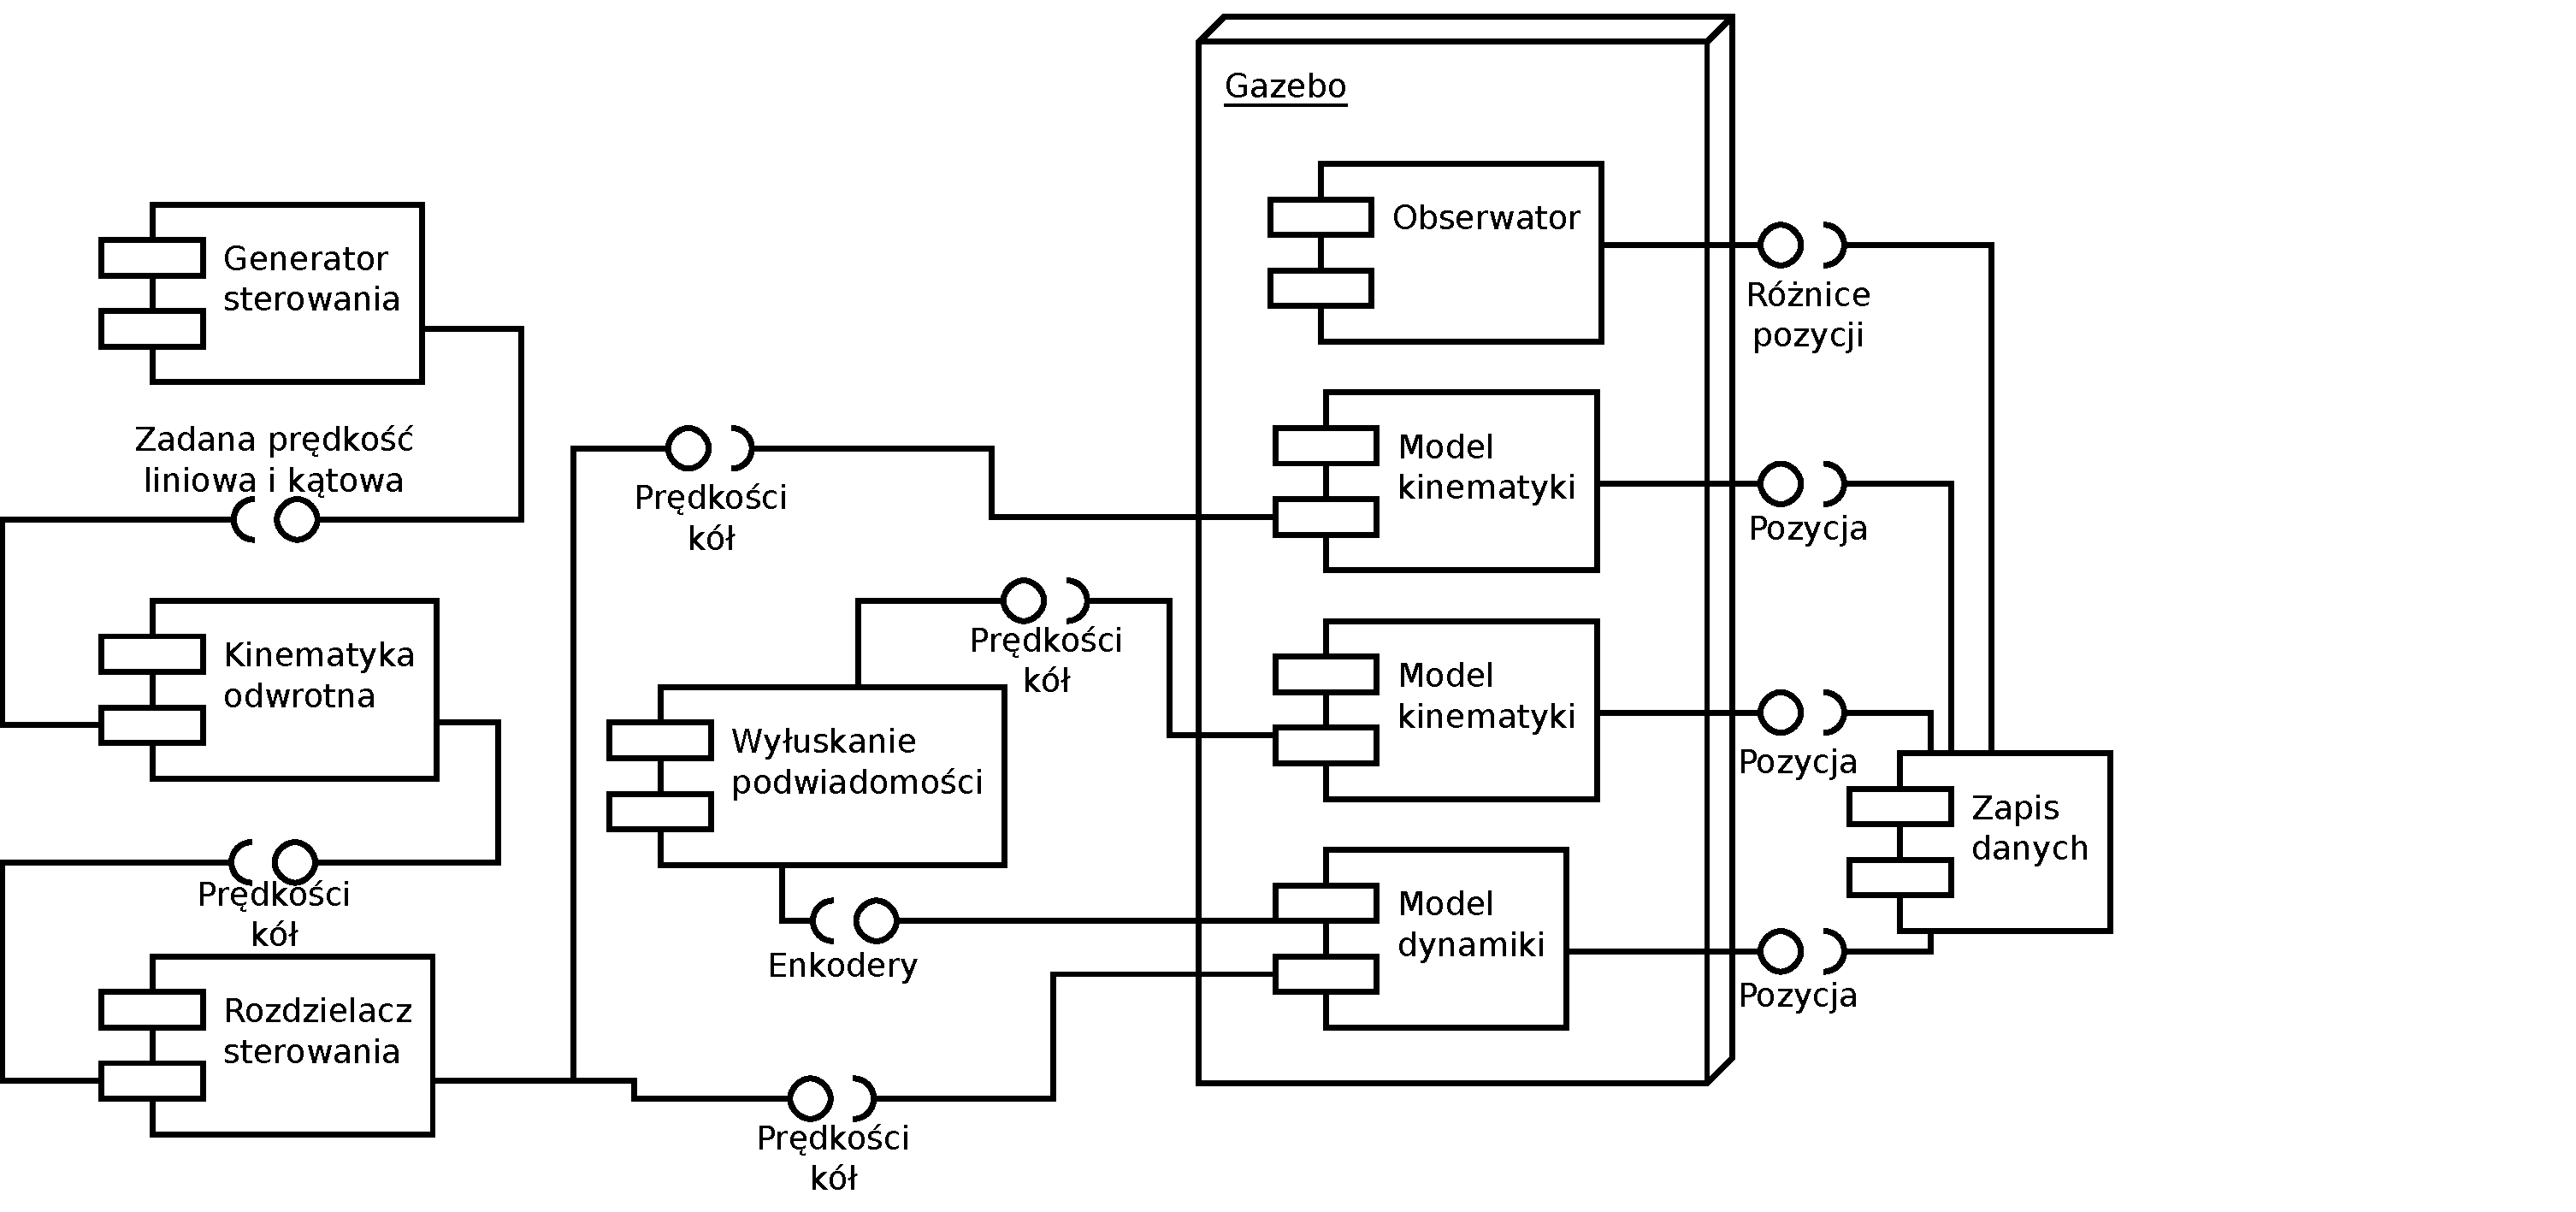
\includegraphics[width=\textwidth]{uml/comparison.pdf}
			\caption{Połączenie pakietów w teście porównującym modele.}
		\label{uml:comparison}
	\end{figure}
	
	\subsection{Porównanie modeli}
		Za pomocą pakietu do nadawania sterowania, opisanego w sekcji \ref{sec:gramofon}, nadano trasę o kształcie przedstawionym na rysunku \ref{plot:comparison_xy}.
		W tym teście robot kolejno poruszał się:
		\begin{enumerate}
			\item W przód z prędkością 0,25 \si{\metre\per\second} przez 5 \si{\second}.
			\item W prawo z prędkością $\pi/32$ \si{\metre\per\second} oraz prędkością kątową o $\pi/32$ \si{\radian\per\second} wokół osi Z, przez 8 \si{\second}.
			\item W tył z tą samą prędkością i przez ten sam czas, jak w punkcie 1.
			\item W prawo z prędkością $\pi/16$ \si{\metre\per\second} oraz prędkością kątową $\pi/32$ \si{\radian\per\second} wokół osi Z, przez 8 \si{\second}.
		\end{enumerate}
		Powyższe akcje wykonał czterokrotnie.
		
		\begin{figure}[H]
			\centering
			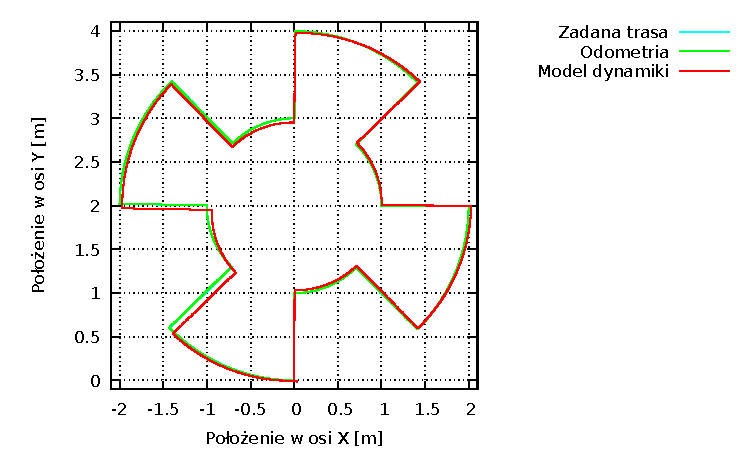
\includegraphics[width=\textwidth]{plots/comparison_xy.pdf}
				\caption{Trasa modelu platformy w teście porównującym modele. Różnica między zadaną trasą, a trasą wyznaczoną przez enkodery, jest niewielka.}
			\label{plot:comparison_xy}
		\end{figure}
		
		\begin{figure}[H]
			\centering
			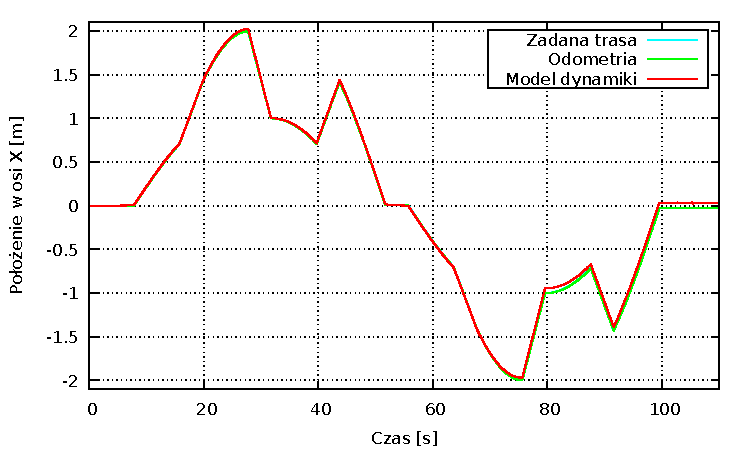
\includegraphics[width=\textwidth]{plots/comparison_xt.pdf}
				\caption{Składowa pozycji modelu wzdłuż osi X w czasie.}
			\label{plot:comparison_xt}
		\end{figure}
		
		\begin{figure}[H]
			\centering
			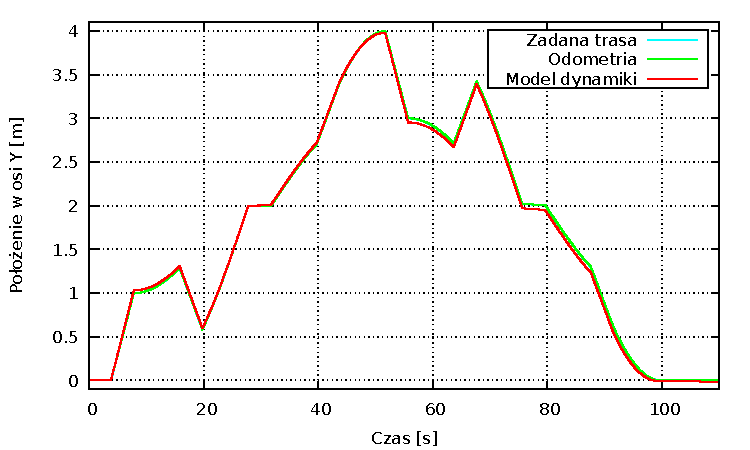
\includegraphics[width=\textwidth]{plots/comparison_yt.pdf}
				\caption{Składowa pozycji modelu wzdłuż osi Y w czasie.}
			\label{plot:comparison_yt}
		\end{figure}
		
		\subsubsection{Dokładność odometrii}
			\label{sec:test_odometry}
			Trasa obliczana na podstawie prędkości kątowej kół, byłaby identyczna do zadanej trasy w przypadku gdyby koła obracałyby się dokładnie z zadanymi prędkościami kątowymi.
			To wymagałoby, aby silniki kół posiadały nieskończony moment siły, lub na tyle duży, aby opór obrotu, spowodowany tarciem, nie wpływał 
			znacząco na ich prędkość kątową. Innymi słowy, nawet jeśli platforma uderzyłaby w przeszkodę, koła nadal powinny obracać się zgodnie z zadanymi wartościami.
			To nie oznacza, że rzeczywista trasa robota jest zgodna z obliczoną z odometrii, gdyż uwzględnia także poślizgi kół, czego enkodery nie są w stanie wykryć.
			
			Różnice w pozycji zadanej, a pozycji obliczonej za pomocą danych wygenerowanych przez enkodery biorą się z tego, że
			silniki mogą nie mieć wystarczającej mocy, aby nadać kołom odpowiednie prędkości i przeciwdziałać oporom.
			Ponieważ założono dużą moc silników, jak zostało to opisane w sekcji \ref{sec:motors}, modelowane koła są mniej podatne na opory, a co za tym idzie, 
			ich prędkość będzie bardziej zbliżona do prędkości zadanej i także trasa wyznaczona w ten sposób z odometrii będzie niemalże pokrywać się z zadaną trasą.
			
			Zauważalne różnice pomiędzy przebiegami trasy odometrycznej i zadanej pojawiają się przy wywoływaniu dużych przyspieszeń i poślizgów na modelu platformy.
			
		\subsubsection{Trasa modelu dynamiki}
			Różnica pomiędzy położeniem modelu dynamiki, a kinematyki (położenia zgodnego z zadaną trasą), rośnie w czasie.
			Jest tak na skutek błędów numerycznych maszyny do symulacji fizyki, braku systemu operacyjnego czasu rzeczywistego, braku zamodelowania wszystkich oporów i skomplikowanej budowy modelu.
			Model dynamiki uwzględnia współczynniki tarcia kół o podłoże i jest w stanie modelować ich poślizgi.
			
			\begin{figure}[h]
				\centering
				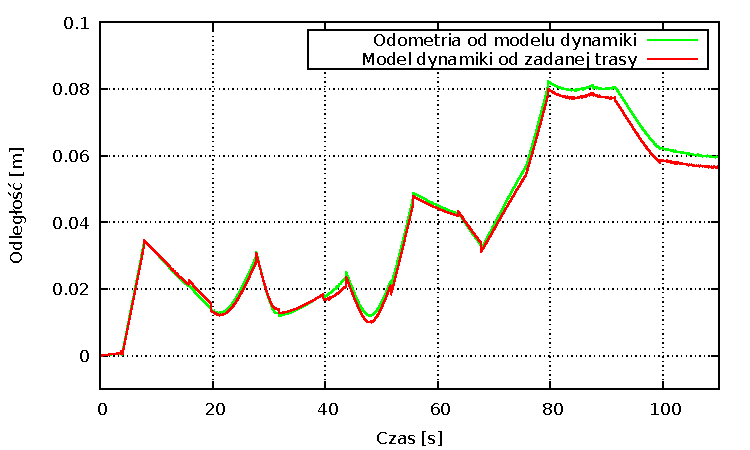
\includegraphics[width=\textwidth]{plots/comparison_dt.pdf}
					\caption{Różnica pomiędzy położeniem modelu dynamiki i modelem kinematyki modelującym zadaną pozycję i pozycję odometryczną.}
				\label{plot:comparison_dt}
			\end{figure}
			
			\begin{figure}[h]
				\centering
				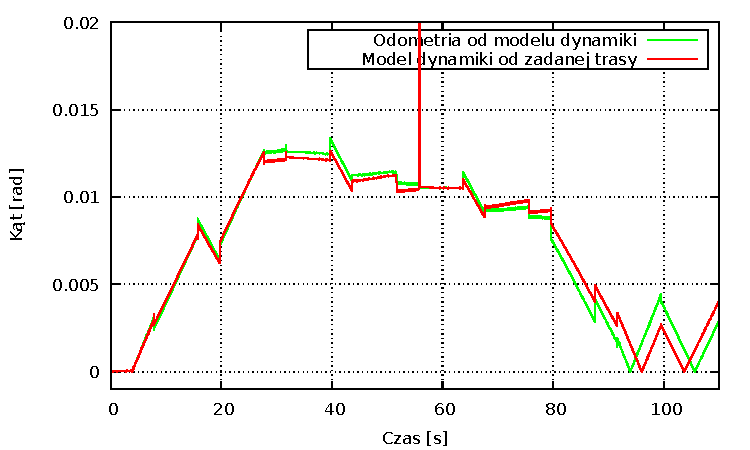
\includegraphics[width=\textwidth]{plots/comparison_at.pdf}
					\caption{Różnica pomiędzy orientacją modelu dynamiki i modelem kinematyki modelującym zadaną pozycję i pozycję odometryczną.}
				\label{plot:comparison_at}
			\end{figure}
			
		\subsubsection{Zachowanie się modelu dynamiki}
			Na wykresie \ref{plot:comparison_dt} zamieszczono różnice między położeniami odpowiednich modeli.
			Różnice nie zmieniają się monotonicznie ze względu na zmiany kierunków prędkości liniowej robota i jego prędkości kątowej wokół osi Z.
			Dlatego też, zdarzają się przypadki w których model dynamiki zbliża się do modelu kinematyki (zadanej pozycji) po tym gdy oddalił się od niej już wcześniej.
			
			Różnica pomiędzy wykresami jest mała, gdyż na obie wartości wpływają poślizgi kół w trakcie pokonywania trasy.
			Enkodery są wstanie wykryć zwiększoną siłę tarcia kół o podłoże na skutek obliczenia różnicy zadanego obrotu, a faktycznego.
			Taka zwiększona siła tarcia towarzyszy nagłym zmianom prędkości platformy, tak samo jak poślizg, lecz to nie powoduje że na
			podstawie pomiarów z enkoderów da się bezpośrednio wyznaczyć wartości poślizgu.
			Inaczej mówiąc, przyspieszenia platformy powodują poślizgi i trudności w obrocie kołami na skutek sił tarcia, lecz korzystając z danych z enkoderów można wyznaczyć
			jedynie opory obrotu kół.
			
			Przykładowe różnice pomiędzy wykresami występują na przykład w 15 sekundzie ruchu. 
			W tym miejscu nastąpił nagły zwrot bazy, który spowodował tarcie, a co za tym idzie i zwiększony opór ruchu obrotowego kół.
			Ten opór został wykryty przez enkodery, lecz poślizg nadal wpłynął na pozycję modelu dynamiki w większym stopniu.
			Dlatego też różnica między pozycją odometryczną, a pozycją modelu dynamiki wzrosła mniej, niż różnica pomiędzy pozycją modelu dynamiki, a pozycją wynikającą z zadanej trasy.
			
			Na wykresie \ref{plot:comparison_at} są pokazane różnice pomiędzy kątem obrotu wokół osi Z tych modeli.
			Podobnie, jak w przypadku położenia, bazując na danych z enkoderów, można obliczyć zmiany kierunku ruchu platformy.
			Na zmianę różnicy kąta obrotu nie wpływają jedynie zmiany prędkości kątowej, a również losowy kąt obrotu nadany platformie w przypadku poślizgów.
			Można zauważyć, że różnica między orientacją modelu dynamiki, a orientacją wyliczoną na podstawie odometrii zwykle zmienia się mniej dynamicznie od 
			różnicy między modelem dynamiki, a zadaną pozycją.
			
	\subsection{Powtarzalność testów}
		Zadano modelowi jazdę z różnymi prędkościami po trasie kwadratu, wyznaczona trasa została przedstawiona na rysunku \ref{plot:repetitions_xy}.
		
		\begin{figure}[H]
			\centering
			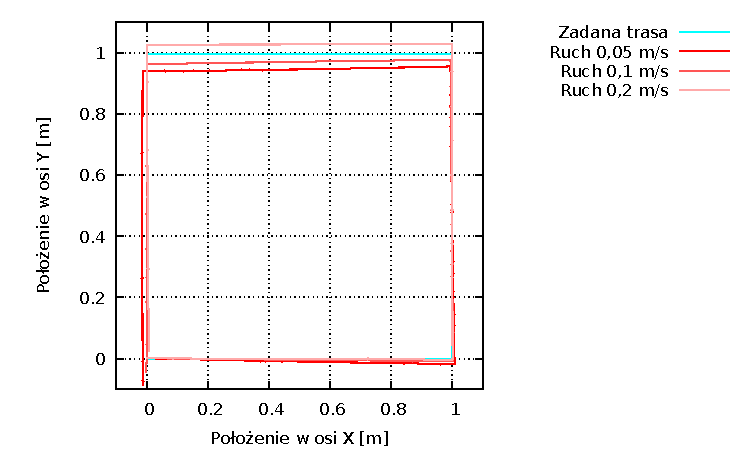
\includegraphics[width=\textwidth]{plots/repetitions_xy.pdf}
				\caption{Trasa modeli platformy, poruszających się z różną prędkością liniową po trasie kwadratu. W tym eksperymencie nie nadano prędkości kątowej.}
			\label{plot:repetitions_xy}
		\end{figure}
		
		Eksperyment pokazuje, że zależnie od prędkości przejazdu, mogą występować niedokładności ruchu. Dzieje się to głównie w kierunku Y, gdyż ruch
		platformy w kierunku X jest zawsze podobny. Im wolniej platforma się porusza, tym mniejszą odległość pokonuje w odpowiednio dłuższym czasie. 
		Tak jest na skutek wewnętrznego działania maszyny do symulacji fizyki. Potrzeba dokładniejszych testów, aby stwierdzić bezpośredni powód takiego zachowania.
		
		Kilkukrotne wykonanie tego samego eksperymentu pokazuje, że różnica tras pomiędzy przejazdami nie jest aż tak duża.
		 
\section{Porównanie modelu z robotem}
	\subsection{Trasa bez rotacji}
		\label{sec:test_velmobil}
		Za pomocą generatora sterowania, zadano platformie ruch po trasie kwadratu w prędkością 0,1 \si{\metre\per\second}, zaczynając od ruchu wzdłuż osi X.
		Zapisano dane generowane przez enkodery, obliczaną odometrię, pomiary skanerów laserowych oraz samo sterowanie.
		Następnie, używając tych samych danych, przeprowadzono identyczny eksperyment na modelu, łącząc pakiety w sposób pokazany na rysunku \ref{uml:comparison}.
		Korzystając z pakietu \texttt{laser\_scan\_matcher}, obliczono rzeczywistą pozycję platformy, korzystając z danych skanerów laserowych.
		Określenie pozycji jest obarczone błędem, wynikającym
		z błędów pomiarowych czujników, stąd obliczona trasa nie składa się z odcinków i posiada szum.
		Trasy modeli i platformy pokazano na wykresie \ref{plot:velmobil_xy}.
		
		\begin{figure}[H]
			\centering
			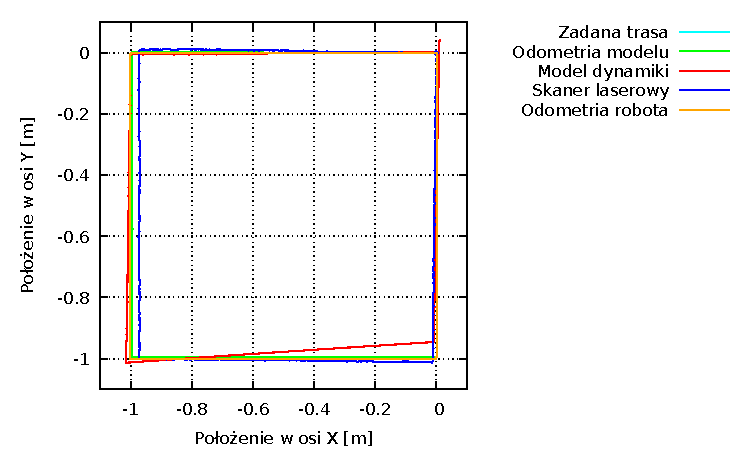
\includegraphics[width=\textwidth]{plots/velmobil_xy.pdf}
				\caption{Trasa modeli robota przy jeździe po trasie kwadratu.}
			\label{plot:velmobil_xy}
		\end{figure}
		
		\begin{figure}[H]
			\centering
			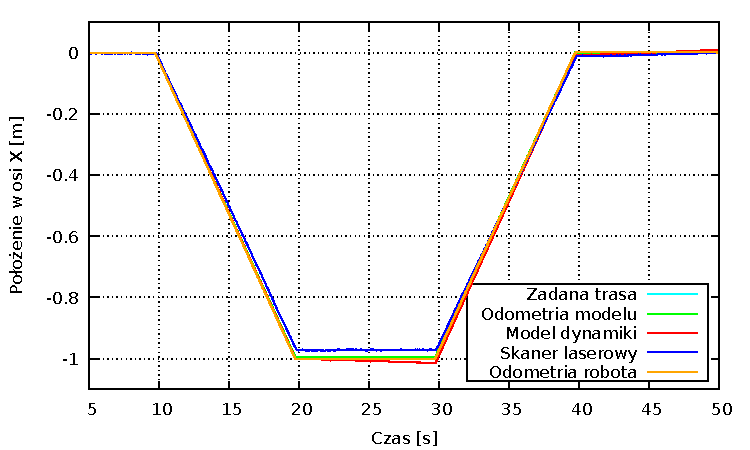
\includegraphics[width=\textwidth]{plots/velmobil_xt.pdf}
				\caption{Składowa pozycji modeli wzdłuż osi X.}
			\label{plot:velmobil_xt}
		\end{figure}
		
		\begin{figure}[H]
			\centering
			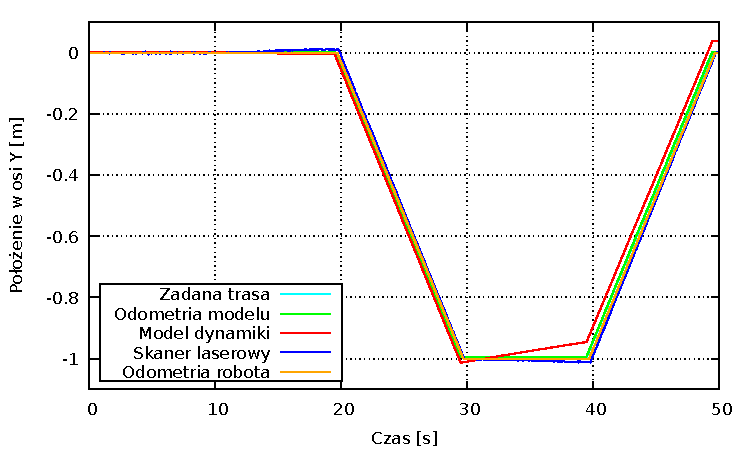
\includegraphics[width=\textwidth]{plots/velmobil_yt.pdf}
				\caption{Składowa pozycji modeli wzdłuż osi Y.}
			\label{plot:velmobil_yt}
		\end{figure}
		
		\begin{figure}[H]
			\centering
			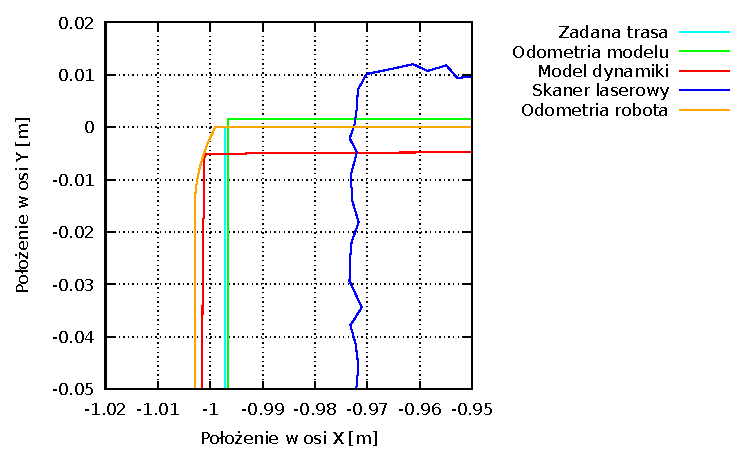
\includegraphics[width=\textwidth]{plots/velmobil_xy_s.pdf}
				\caption{Przybliżenie wykresu \ref{plot:velmobil_xy}}
			\label{plot:velmobil_xy_s}
		\end{figure}
		
		Charakterystyczną cechą wykresu jest to, że robot przejechał mniejszą odległość wzdłuż osi X, niż wzdłuż osi Y.
		Może być to spowodowane różnicą w wyjściowym współczynniku tarcia kół w zależności od wyjściowego wektora prędkości kół.
		Zgodnie z cechą kół, opisaną w sekcji \ref{sec:robot_movement}, rolki kół obracają się z największą prędkością przy ruchu w bok, a co za tym idzie, w ruchu ma udział także
		ich tarcie obrotowe. Przy ruchu w przód, rolki nie obracają się, więc i to dodatkowe tarcie nie wpływa na ruch platformy.
		Dlatego też platforma pokonała mniejszą odległość w jednym z kierunków.
		
		Model dynamiki doznał poślizgu w trakcie 30 sekundy ruchu, która nadała mu niespodziewaną zmianę orientacji, przez co różnica w odległości od zadanej trasy znacząco wzrosła.
		
		\subsubsection{Nagła zmiana kierunku jazdy}
			Na wykresie \ref{plot:velmobil_xy_s} przedstawiono przybliżenie trasy modeli i robota w trakcie drugiego skrętu.
			Opisane niżej cechy są szczególnie dobrze widoczne na wektorowych wykresach w przypadku dokumentu elektronicznego.
			\begin{description}
				\item[Zadana trasa] nie pokrywa się dokładnie z przewidzianą trasą kwadratu, następują jej nieznaczne odchylenia.
				Jest to spowodowane działaniem symulacji i programu generującego sterowanie na systemie operacyjnym, który nie był systemem czasu rzeczywistego.
				Dodatkowo, pakiety sieciowe, zawierające wiadomości ROSa, przesyłane były przez sieć Ethernet, która nie gwarantuje przesyłu w deterministycznym czasie.
				To powoduje, że obliczona trasa nie koniecznie pokrywa się z zadaną trasą. Co więcej, na skutek niedeterministycznego przekazywania wiadomości przez strumienie komunikacyjne w czasie symulacji, każdy model i platforma mogły otrzymać nieco inne sterowanie, a co za tym idzie, różnice pomiędzy ich położeniami mogły być spowodowane tym efektem.
				\item[Odometria modelu] Jak wspomniano w sekcji \ref{sec:test_odometry}, trasa obliczona na jej podstawie niemal pokrywa się z zadaną trasą. 
				Jednakże, w trakcie nagłej zmiany kierunku ruchu, tarcie kół spowodowało nieznaczną różnicę prędkości kół w stosunku do zadanych wartości, co jest 
				wykryte jako ścięcie wykresu w kierunku Y. W przypadku modelu jest ono bardzo niewielkie, ale w tym samym kierunku, jak obliczone przez odometrię robota.
				To oznacza, że model enkoderów działa poprawnie, lecz być może jego parametry, czyli moment siły kół lub tarcie rolek nie są odpowiednio dobrane.
				\item[Model dynamiki] wykazał bezwładność w trakcie ruchu, to znaczy, jego prędkość liniowa w kierunku osi Y nie wzrosła natychmiastowo,
				lecz pod wpływem przyspieszenia, tak samo prędkość w kierunku X, która także nie spadła natychmiast.
				Jest to widoczne jako zaokrąglenie na wykresie.
				Opóźnienie w kierunku X było większe, niż przyspieszenie w kierunku Y, tzn. model szybciej wyhamował składową X prędkości liniowej, niż nadał zadaną składową Y prędkości liniowej, co się objawia jako wydłużenie trasy w danym kącie. Takie samo zachowanie wykazały trasy odometrii.
				\item[Skaner laserowy] Ponieważ pomiar z tego czujnika jest obarczony dużym błędem oraz małą częstotliwością pomiarów, nie można jednoznacznie określić bezpośredniego zachowania platformy w trakcie skrętu.
				\item[Odometria robota] Korzystając z enkoderów, program sterujący platformą obliczył jej pozycję. Nie jest to dokładna pozycja platformy, jaka jest określona przez skaner laserowy, lecz trasa wyznaczona tym sposobem jest zbliżona do zadanej trasy tak samo, jak trasa odometrii modelu. 
				Wykazuje takie same własności w trakcie skrętu, jak jej model, tylko w większym stopniu. Różnica w przyspieszeniu i opóźnieniu robota wskazuje, że 
				robot szybciej hamuje w kierunku X, niż przyspiesza w kierunku Y. Taki sam efekt występuje po drugiej stronie trasy, przy trzecim skręcie, lecz nie w drugim skręcie.
			\end{description}

	\subsection{Trasa z rotacją}
		\label{sec:test_velmobil_rot}
		Sterowanie robotem odbyło się w sposób podobny do testu \ref{sec:test_velmobil}, z tą różnicą, że przy wcześniejszej zmianie kierunku prędkości liniowej obracano platformą o 90° wokół osi Z. To znaczy, że platforma poruszała się w prawo z prędkością 0,1 \si{\metre\per\second}, a następnie obróciła o 90° 
		z prędkością kątową $\pi/20$ \si{\radian\per\second} i ponownie poruszała się w kierunku -X lokalnego układu współrzędnych.
		Trasa takiego przejazdu została przedstawiona na wykresie \ref{plot:velmobil_rot_xy}.
		Można na niej zauważyć poślizg przy ruszaniu platformy, który nadał jej losowy kąt obrotu.
		
		\begin{figure}[H]
			\centering
			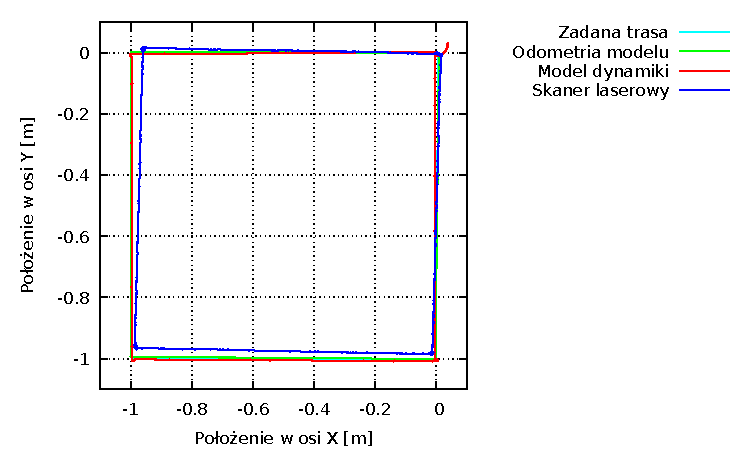
\includegraphics[width=\textwidth]{plots/velmobil_rot_xy.pdf}
				\caption{Trasa modeli robota przy jeździe po trasie kwadratu z nadaniem prędkości kątowej wokół osi Z.}
			\label{plot:velmobil_rot_xy}
		\end{figure}
		
		\begin{figure}[H]
			\centering
			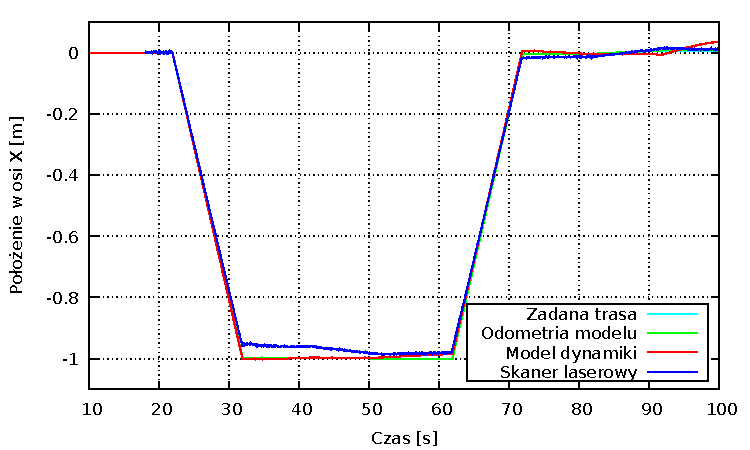
\includegraphics[width=\textwidth]{plots/velmobil_rot_xt.pdf}
				\caption{Składowa pozycji modeli wzdłuż osi X.}
			\label{plot:velmobil_rot_xt}
		\end{figure}
		
		\begin{figure}[H]
			\centering
			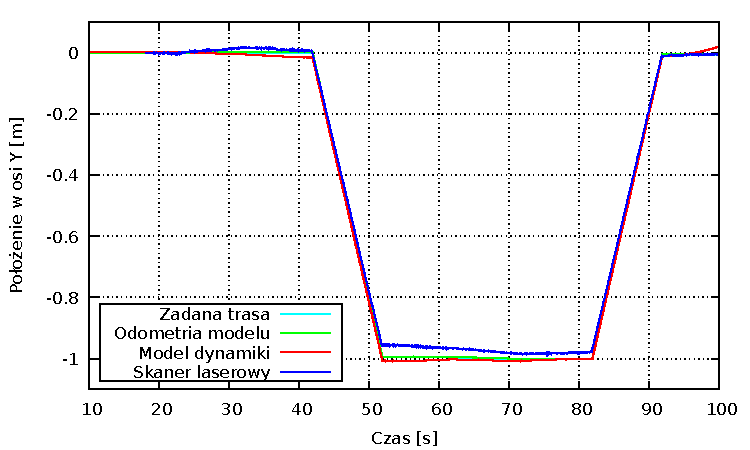
\includegraphics[width=\textwidth]{plots/velmobil_rot_yt.pdf}
				\caption{Składowa pozycji modeli wzdłuż osi Y.}
			\label{plot:velmobil_rot_yt}
		\end{figure}
		
		\begin{figure}[H]
			\centering
			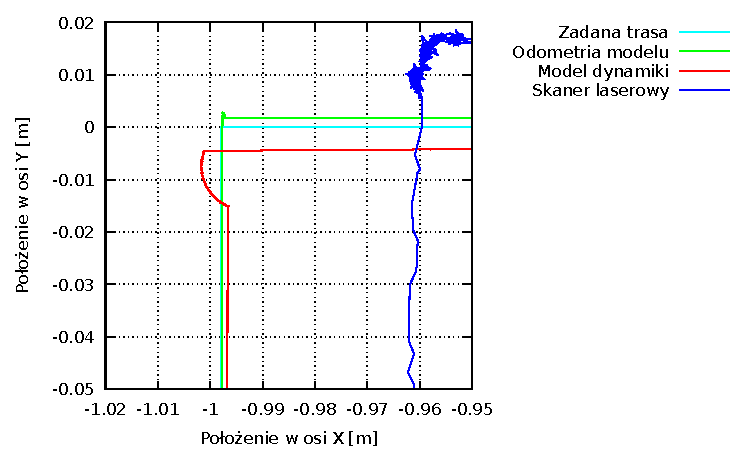
\includegraphics[width=\textwidth]{plots/velmobil_rot_xy_s.pdf}
				\caption{Przybliżenie wykresu \ref{plot:velmobil_rot_xy}}
			\label{plot:velmobil_rot_xy_s}
		\end{figure}
	
		W tym przypadku nie ma informacji o odometrii wygenerowanej przez robota, gdyż nie obsługuje ona poprawnie rotacji platformy.
		
		Na przybliżeniu wykresu (rysunek \ref{plot:velmobil_rot_xy_s}) widać moment jak model dojechał do odpowiedniej pozycji i zaczął się obracać wokół osi Z. 
		Wykres pokazuje, że obrót następował wokół punktu znajdującego się o około 0,5 \si{\centi\metre} na prawo od środka modelu platformy.
		Nie jest wiadome, dlaczego tak się stało, gdyż model jest zdefiniowany symetrycznie, a środek układu współrzędnych, względem którego rysowany jest wykres, znajduje się 
		na środku platformy.
		Według enkoderów, punkt obrotu znajdował się z kolei na lewo od środka platformy.
		Takie zachowanie może być spowodowane na przykład asymetrią siatki definiującej kształt platformy, kolejnością obliczeń wykonywanych przy symulowaniu ogniw 
		obiektu lub innymi własnościami maszyny do symulacji fizyki.
	
\section{Jednostka inercyjna}
	\label{sec:test_imu}
	W trakcie powyższych testów zabrano również dane wygenerowane przez jednostkę inercyjną oraz jej model.
	\subsection{Akcelerometr}
		Ten czujnik zmierzył przyspieszenia modelu w trakcie testu \ref{sec:test_velmobil}.
		
		\begin{figure}[H]
			\centering
			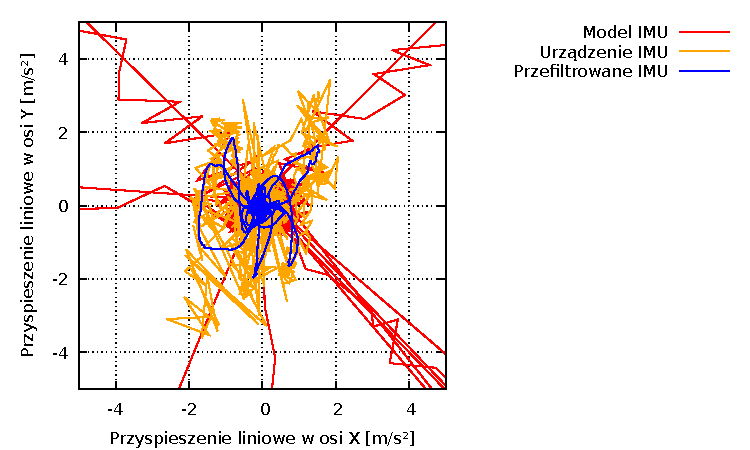
\includegraphics[width=\textwidth]{plots/imu_xy.pdf}
				\caption{Porównanie odczytów pomiaru przyspieszenia liniowego jednostki inercyjnej, jej modelu i filtra redukującego szum.}
			\label{plot:imu_xy}
		\end{figure}
		
		W trakcie testu następowały kolejne przyspieszenia i opóźnienia bazy w zadanych kierunkach, to widać jako impulsy na wykresie \ref{plot:imu_xy}.
		Na początku platforma zaczęła poruszać się w kierunku -X i w tą stronę zostało nadane pierwsze przyspieszenie.
		Nie jest znana jego dokładna wielkość, gdyż zadany kierunek prędkości zmienił się w ciągu jednej wiadomości.
		
		Drugi impuls został wygenerowany w trakcie pierwszego skrętu bazy.
		Zadziałało przyspieszenie zmieniające kierunek prędkości liniowej platformy o 90°, co oznacza że impuls jest obrócony o 45° względem układu współrzędnych.
		Impuls wystąpił w kierunku (X,-Y). 
		Jest to wypadkowa przyspieszenia bazy w kierunku -Y i opóźnienia w kierunku poprzedniego kierunku jazdy, czyli -X.
		
		Podobna zmiana prędkości nastąpiła jeszcze dwa razy, generując kolejne, symetryczne impulsy.
		
		Na koniec platforma zatrzymała się, generując opóźnienie w kierunku Y, co także widać na wykresie w postaci przyspieszenia w przeciwnym kierunku.
		
		Porównując dane wygenerowane przez jednostkę inercyjną nie widać zależności, jednak zastosowanie prostego uśrednienia pakietem opisanym w sekcji \ref{sec:odszumiacz} powoduje, że impulsy wygenerowane przez robota również są widoczne. Każda uśredniona wartość jest średnią z 40 poprzednich.
		
		Po przefiltrowaniu danych z robota, można zaobserwować jak każdy impuls ma kształt półksiężyca, na początku każdej zmiany prędkości opóźnienie ma kierunek równoległy do wektora prędkości, zatrzymując robota, następnie wolniejsze przyspieszenie nadaje nowy kierunek, a potem następuje reakcja korpusu i gasnące drgania w nowym kierunku. 
		Zamodelowanie tej własności mogłoby okazać się bardzo trudne, prawdopodobnie należałoby nadać dodatkowe ogniwa do robota i połączyć je więzami sprężynowymi.
		
		Szum, jakimi są obarczone zamodelowane dane spowodowany jest potrzebą różniczkowania prędkości liniowej modelu, obliczanej dyskretnie przez maszynę do symulacji fizyki. 
		Wartości mas i momentów bezwładności ogniw modelu mocno wpływają na kształt impulsów, kolerację
		osi i szum na wykresie. 
		Nie jest technologicznie możliwe zamodelowanie jednostki inercyjnej pozbawionej szumu ze względu na błędy numeryczne, algorytmy użyte w maszynie
		symulującej fizykę i system operacyjny na którym pracuje symulator.
		
		\begin{figure}[H]
			\centering
			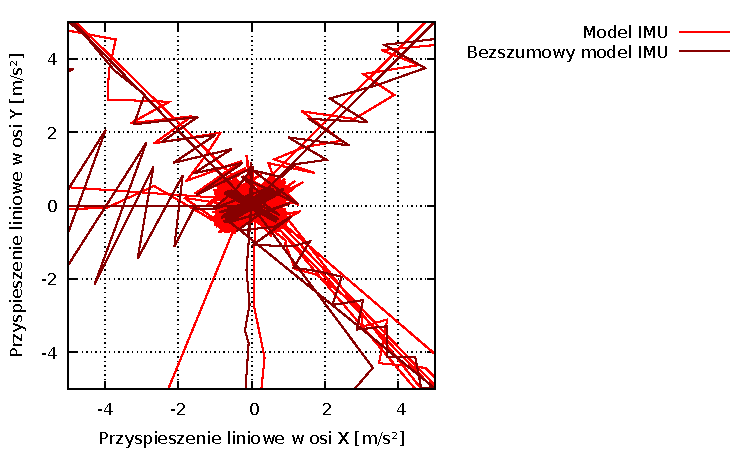
\includegraphics[width=\textwidth]{plots/imu_xy_n.pdf}
				\caption{Porównanie odczytów pomiaru przyspieszenia liniowego modeli jednostki inercyjnej z dodanym szumem i bez.}
			\label{plot:imu_xy_n}
		\end{figure}
		
		Na wykresie \ref{plot:imu_xy} widać szum generowany przez jednostkę inercji w trakcie ruchu jednostajnego. Jest on mniejszy od niedokładności generowanych
		przez model. Jednakże, w trakcie działania przyspieszenia, model jednostki inercyjnej wygenerował większy impuls, niż urządzenie.
		Do wykrycia kierunków impulsów nie potrzebna jest filtracja danych, ale taka filtracja okazała się niezbędna w przypadku danych zebranych z jednostki inercyjnej.
		
		Aby przybliżyć zachowanie się modelu jednostki inercyjnej w trakcie ruchu z prędkością jednostajną, do odczytów urządzenia, dodano dodatkowy szum o rozkładzie normalnym.
		Jego parametry określone są w tabeli \ref{tab:imu_noise}.
		Na rysunku \ref{plot:imu_xy_n} przedstawiono porównanie generowanych przez model danych z szumem i bez.
		Można zauważyć silną korelację modelu jednostki inercyjnej w zależności od kierunku prędkości liniowej robota. 
		Korelacja jest także silnie uzależniona od parametrów modelu dynamiki. Występują bazowe drgania w dwóch kierunkach.
		Niestety, amplituda bazowych drgań w modelowanym czujniku jest większa niż amplituda szumu rzeczywistej jednostki, w dodatku występuje korelacja wzdłuż dwóch prostych.
		Widać to na wykresach przebiegu czasowego \ref{plot:imu_yt} i \ref{plot:imu_xt}.
		
		\begin{figure}[H]
			\centering
			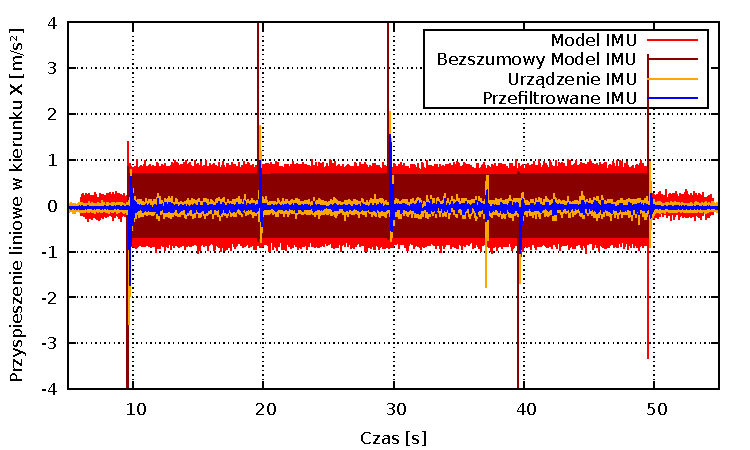
\includegraphics[width=\textwidth]{plots/imu_xt.pdf}
				\caption{Porównanie składowej X pomiarów przyspieszenia liniowego jednostki inercyjnej, jej modelu i filtra redukującego szum.}
			\label{plot:imu_xt}
		\end{figure}
		
		\begin{figure}[H]
			\centering
			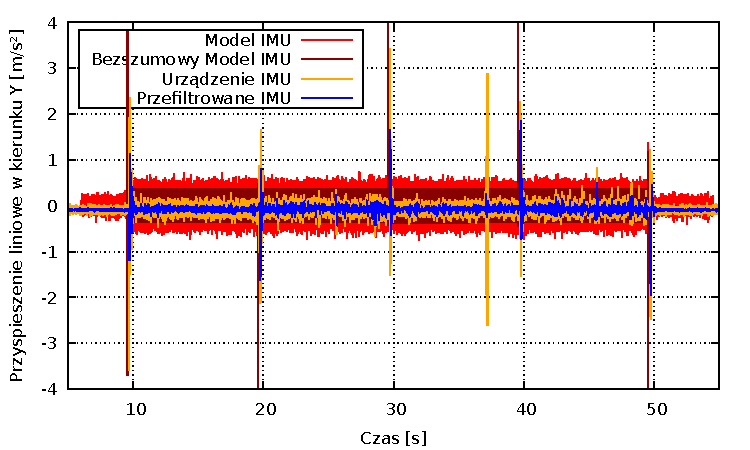
\includegraphics[width=\textwidth]{plots/imu_yt.pdf}
				\caption{Porównanie składowej Y pomiarów przyspieszenia liniowego jednostki inercyjnej, jej modelu i filtra redukującego szum.}
			\label{plot:imu_yt}
		\end{figure}
		
		Aby użyć tego czujnika do obliczania pozycji, trzeba wpierw użyć bardziej zaawansowanego algorytmu odszumiającego i wyprowadzić eksperymentalnie zależności pomiędzy czujnikami
		osi (macierz kowariancji).
		
		Na wykresach \ref{plot:imu_xt} i \ref{plot:imu_yt} widać jak w około 15 sekundzie ruchu na platformę zadziałała nagła zmiana prędkości liniowej.
		Wykres przebiegu trasy nie wskazuje, jakoby zdarzyła się tam nagła zmiana prędkości.
	
	\subsection{Żyroskop}
		Czujnik prędkości kątowej korzysta z żyroskopu i zwraca prędkość kątową we wszystkich trzech osiach.
		Ponieważ jednak platforma porusza się po płaskim terenie, wymagany jest jedynie czujnik mierzący obrót wokół osi Z, czyli w górę.
		Drugą osią wykresu może być zatem czas nadania pakietu. Te dane zostały zebrane w trakcie testu \ref{sec:test_velmobil_rot}.
		
		\begin{figure}[H]
			\centering
			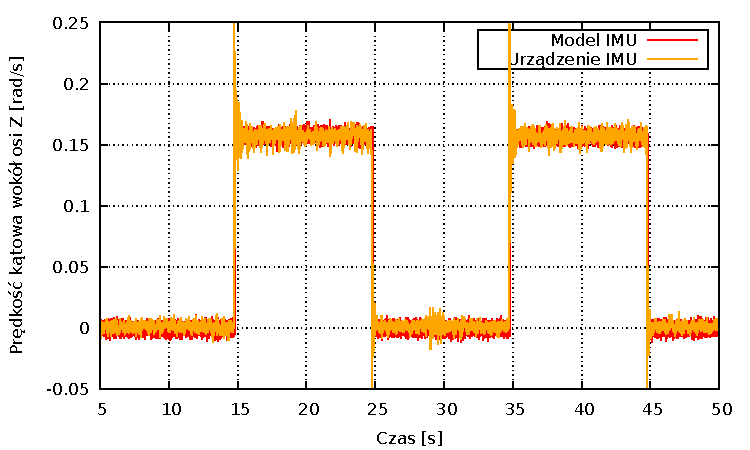
\includegraphics[width=\textwidth]{plots/angimu_at.pdf}
				\caption{Porównanie prędkości kątowej wokół osi Z, wygenerowanej przez jednostkę inercyjną i jej model.}
			\label{plot:angimu_at}
		\end{figure}
		
		\begin{figure}[h]
			\centering
			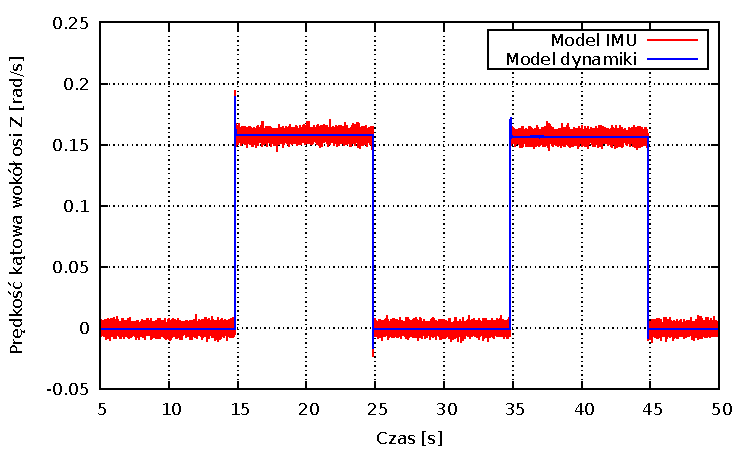
\includegraphics[width=\textwidth]{plots/angimu_at_w.pdf}
				\caption{Porównanie danych wygenerowanych przez model jednostki inercyjnej i prędkości kątowej wokół osi Z modelu.}
			\label{plot:angimu_at_w}
		\end{figure}
		
		Ponieważ maszyna do symulacji fizyki wewnętrznie posiada informację o prędkościach obiektów, model tego czujnika po prostu zwraca gotowe dane. 
		To powoduje, że praktycznie pozbawiony jest szumu, co można zauważyć na wykresie \ref{plot:angimu_at_w}.
		Aby zatem polepszyć jakość symulacji, dodano sztuczny szum do generowanych danych, zgodnie z tabelą \ref{tab:imu_noise}.
		W ten sposób wykresy są do siebie bardziej zbliżone.
		
		Jednak niektórych własności czujnika nie da się zamodelować tak łatwo. Po pierwsze, szum czujnika nie do końca ma rozkład normalny.
		Z wykresu można zobaczyć, że dane prawdopodobnie korelują z częstotliwościami obrotu kół.
		Dodatkowo, nagła zmiana prędkości kątowej powoduje zauważalny skok na wykresie, co w symulowanych danych jest znacznie mniej widoczne.
		Może być to spowodowane drganiem robota przy nagłych zmianach prędkości kątowej, co nie jest uwzględnione w modelu.
		
		
		
	
	

%TODO różnica współczynników tracia w bok i do przodu
